\documentclass[12pt, a4paper]{article}
\usepackage{fontspec}
\usepackage{xeCJK}
\usepackage{hyperref}
\setCJKmainfont{微軟正黑體}
\XeTeXlinebreaklocale "zh"
\XeTeXlinebreakskip = 0pt plus 1pt
\usepackage{enumerate}
\usepackage{graphicx}
\usepackage{amsmath}
\usepackage[tmargin = 4cm]{geometry}
\date{}
\title{\vspace{-3.0cm} Robotics : Assignment 2 \\ \vspace{0.5cm}}
\author{\normalsize B03902062 資工三 \hspace{0cm} 董文捷}
\begin{document}
\maketitle

\noindent {\bf PART A}
\begin{enumerate}[(1)]

\item
{\bf According to ER-7 arm, draw the link coordinate diagram using D-H convention.} \\
\newline
Link 1 \hspace{6cm} Link 2 \\
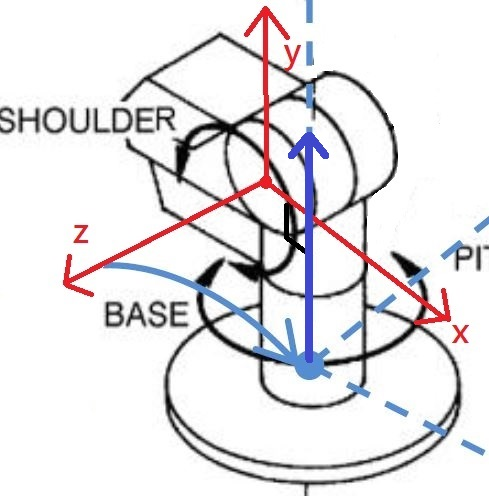
\includegraphics[scale = 0.5]{link1.JPG}
\hspace{1cm}
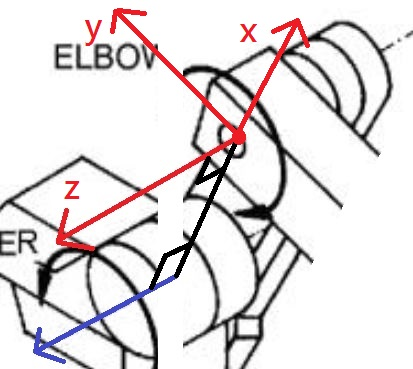
\includegraphics[scale = 0.5]{link2.JPG} \\
\newline
Link 3 \hspace{6cm} Link 4 \\
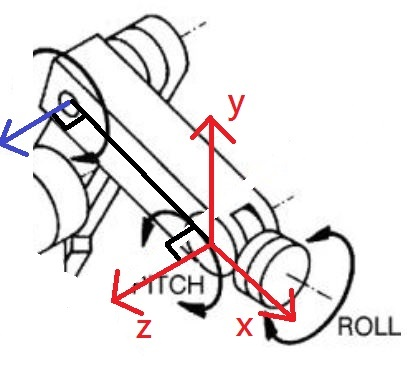
\includegraphics[scale = 0.5]{link3.JPG}
\hspace{1cm}
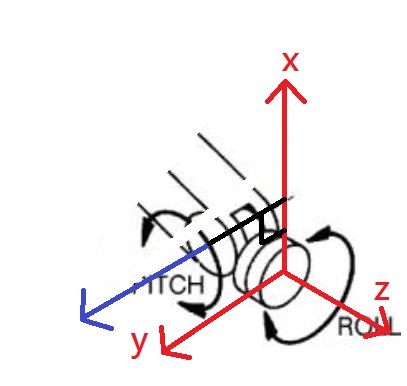
\includegraphics[scale = 0.5]{link4.JPG} \\

\newpage
\item
{\bf According to the 2 joints shown in Fig 1, please define the four D-H parameters.} \\
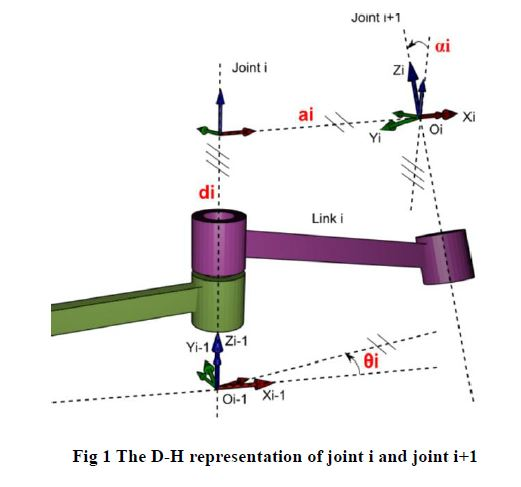
\includegraphics{fig1.JPG}
\begin{itemize}
\item 
$\alpha_i$ = the angle between $z_{i-1}$ and $z_i$ measured about common normal $x_i$
\item
$a_i$ = the distance from $z_{i-1}$ to $z_i$ measured along common normal $x_i$
\item
$d_i$ = the distance from $x_{i-1}$ to $x_i$ measured along $z_{i - 1}$
\item
$\theta_i$ = the angle between $x_{i-1}$ and $x_i$ measured about $z_{i - 1}$
\end{itemize}

\item
{\bf Find the kinematics parameters of ER-7 and fill the table below: } \\
\begin{tabular}[t]{|ccccc|}
\hline 
Joint & $\theta_i$ (rad) & $d_i$ (mm) & $a_i$ (mm) & $\alpha_i$ (rad) \\
\hline
1 & $\theta_1$ & $358.5$ & $50$ & $\frac{\pi}{2}$ \\
\hline
2 & $\theta_2$ & $-35$ & $300$ & 0 \\
\hline
3 & $\theta_3$ & $0$ & $350$ & 0 \\
\hline
4 & $\theta_4$ & $0$ & $0$ & $\frac{\pi}{2}$ \\
\hline
5 & $\theta_5$ & $251$ & $0$ & $0$ \\
\hline
\end{tabular} 

\end{enumerate}

\newpage
\noindent {\bf PART B} \\
The transformation matrix from joint $i - 1$ to joint $i$ based on the {\it DH convention} is given by \\
${ }^{i-1} T_{i} =
\begin{bmatrix}
\cos \theta_i & -\cos \alpha_i \sin \theta_i & \sin \alpha_i \sin \theta_i & a_i \cos \theta_i \\
\sin \theta_i & \cos \alpha_i \cos \theta_i & -\sin \alpha_i \cos \theta_i & a_i \sin \theta_i \\
0 & \sin \alpha_i & \cos \alpha_i & d_i \\
0 & 0 & 0 & 1 \\
\end{bmatrix}$
\\
By taking DH parameters found in {\bf PART A(3)}, we can get 
\\
\hspace*{-0.4cm} ${ }^{0} T_{1} =
\begin{bmatrix}
\cos \theta_1 & -\cos \frac{\pi}{2} \sin \theta_1 & \sin \frac{\pi}{2} \sin \theta_1 & 50 \cos \theta_1 \\
\sin \theta_1 & \cos \frac{\pi}{2} \cos \theta_1 & -\sin \frac{\pi}{2} \cos \theta_1 & 50 \sin \theta_1 \\
0 & \sin \frac{\pi}{2} & \cos \frac{\pi}{2} & 358.5 \\
0 & 0 & 0 & 1 \\
\end{bmatrix}$
= 
$\begin{bmatrix}
\cos \theta_1 & 0 & \sin \theta_1 & 50 \cos \theta_1 \\
\sin \theta_1 & 0 & - \cos \theta_1 & 50 \sin \theta_1 \\
0 & 1 & 0 & 358.5 \\
0 & 0 & 0 & 1 \\
\end{bmatrix}$

\hspace*{-1cm} ${ }^{1} T_{2} =
\begin{bmatrix}
\cos \theta_2 & -\cos 0 \sin \theta_2 & \sin 0 \sin \theta_2 & 300 \cos \theta_2 \\
\sin \theta_2 & \cos 0 \cos \theta_2 & -\sin 0 \cos \theta_2 & 300 \sin \theta_2 \\
0 & \sin 0 & \cos 0 & -35 \\
0 & 0 & 0 & 1 \\
\end{bmatrix}$
= 
$\begin{bmatrix}
\cos \theta_2 & -\sin \theta_2 & 0 & 300 \cos \theta_2 \\
\sin \theta_2 & \cos \theta_2 & 0 & 300 \sin \theta_2 \\
0 & 0 & 1 & -35 \\
0 & 0 & 0 & 1 \\
\end{bmatrix}$

\hspace*{-1cm} ${ }^{2} T_{3} =
\begin{bmatrix}
\cos \theta_3 & -\cos 0 \sin \theta_3 & \sin 0 \sin \theta_3 & 350 \cos \theta_3 \\
\sin \theta_3 & \cos 0 \cos \theta_3 & -\sin 0 \cos \theta_3 & 350 \sin \theta_3 \\
0 & \sin 0 & \cos 0 & 0 \\
0 & 0 & 0 & 1 \\
\end{bmatrix}$
= 
$\begin{bmatrix}
\cos \theta_3 & -\sin \theta_3 & 0 & 350 \cos \theta_3 \\
\sin \theta_3 & \cos \theta_3 & 0 & 350 \sin \theta_3 \\
0 & 0 & 1 & 0 \\
0 & 0 & 0 & 1 \\
\end{bmatrix}$

\hspace*{-1cm} ${ }^{3} T_{4} =
\begin{bmatrix}
\cos \theta_4 & -\cos \frac{\pi}{2} \sin \theta_4 & \sin \frac{\pi}{2} \sin \theta_4 & 0 \cos \theta_4 \\
\sin \theta_4 & \cos \frac{\pi}{2} \cos \theta_4 & -\sin \frac{\pi}{2} \cos \theta_4 & 0 \sin \theta_4 \\
0 & \sin \frac{\pi}{2} & \cos \frac{\pi}{2} & 0 \\
0 & 0 & 0 & 1 \\
\end{bmatrix}$
= 
$\begin{bmatrix}
\cos \theta_4 & 0 & \sin \theta_4 & 0 \\
\sin \theta_4 & 0 & - \cos \theta_4 & 0 \\
0 & 1 & 0 & 0 \\
0 & 0 & 0 & 1 \\
\end{bmatrix}$

\hspace*{-1cm} ${ }^{4} T_{5} =
\begin{bmatrix}
\cos \theta_5 & -\cos 0 \sin \theta_5 & \sin 0 \sin \theta_5 & 0 \cos \theta_5 \\
\sin \theta_5 & \cos 0 \cos \theta_5 & -\sin 0 \cos \theta_5 & 0 \sin \theta_5 \\
0 & \sin 0 & \cos 0 & 251 \\
0 & 0 & 0 & 1 \\
\end{bmatrix}$
= 
$\begin{bmatrix}
\cos \theta_5 & -\sin \theta_5 & 0 & 0 \\
\sin \theta_5 & \cos \theta_5 & 0 & 0 \\
0 & 0 & 1 & 251 \\
0 & 0 & 0 & 1 \\
\end{bmatrix}$

\newpage
\noindent {\bf PART C}
\begin{enumerate}[(1)]

\item
Multiplying these matrices to form a transformation matrix from the base frame to the gripper tip : \\
${ }^{3} T_{5} = { }^{3} T_{4} \times { }^{4} T_{5} = 
\begin{bmatrix}
c_4 c_5 & -c_4  s_5 & s_4 & 251 s_4 \\
c_5 s_4 & -s_4  s_5 & -c_4 & -251 c_4 \\
s_5 & c_5 & 0 & 0 \\
0 & 0 & 0 & 1 \\
\end{bmatrix}$ 
\\
${ }^{2} T_{5} = { }^{2} T_{3} \times { }^{3} T_{5} = 
\begin{bmatrix}
c_{34} c_5 & -c_{34}  s_5 & s_{34} & 350 c_3 + 251 s_{34} \\
s_{34} c_5 & -s_{34}  s_5 & -c_{34} & 350 s_3 - 251 c_{34} \\
s_5 & c_5 & 0 & 0 \\
0 & 0 & 0 & 1 \\
\end{bmatrix}$
\\
${ }^{1} T_{5} = { }^{1} T_{2} \times { }^{2} T_{5} = 
\begin{bmatrix}
c_{234}c_5 & -c_{234}s_5 & s_{234} & 300c_2+350c_{23}+251s_{234} \\
s_{234}c_5 & -s_{234}s_5 & -c_{234} & 300s_2+350s_{23}-251c_{234} \\
s_5 & c_5 & 0 & -35 \\
0 & 0 & 0 & 1 \\
\end{bmatrix}
$ 
\\
${ }^{0} T_{5} = { }^{0} T_{1} \times { }^{1} T_{5}$ = \\
\scalebox{0.8}{
$\begin{bmatrix}
s_1s_5 + c_1c_{234}c_5 & s_1c_5 - c_1c_{234}s_5 & c_1s_{234} & -35s_1 + c_1(50 + 300c_2 + 350c_{23} + 251s_{234}) \\
s_1c_{234}c_5 - c_1s_5 & -c_1c_5 - c_{234}s_1s_5 & s_1s_{234} & 35c_1 + s_1(50 + 300c_2 + 350c_{23} + 251s_{234}) \\
s_{234}c_5 & -s_{234}s_5 & -c_{234} & 300s2 + 350s_{23} - 251c_{234} + 358.5 \\
0 & 0 & 0 & 1 \\
\end{bmatrix}$
}

For $Z-Y-X$ Euler angles, the rotation matrix is \\
${ }^{A} R_{B} = 
\begin{bmatrix}
\cos \phi \cos \theta & \cos \phi \sin \theta \sin \psi - \sin \phi \cos \psi & \cos \phi \sin \theta \cos \psi + \sin \phi \sin \psi \\
\sin \phi \cos \theta & \sin \phi \sin \theta \sin \psi + \cos \phi \cos \psi & \sin \phi \sin \theta \cos \psi - \cos \phi \sin \psi \\
-\sin \theta & \cos \theta \sin \psi &  \cos \theta \cos \psi \\
\end{bmatrix}$

${ }^{0} T_{5} = P =
\begin{bmatrix}
c_\phi c_\theta & c_\phi s_\theta s_\psi - s_\phi c_\psi & c_\phi s_\theta c_\psi + s_\phi s_\psi & x\\ 
s_\phi c_\theta & s_\phi s_\theta s_\psi + c_\phi c_\psi & s_\phi s_\theta c_\psi - c_\phi s_\psi & y\\
-s_\theta & c_\theta s_\psi &  c_\theta c_\psi & z\\
0 & 0 & 0 & 1\\
\end{bmatrix}$

For inverse kinematics, \\
$[{ }^{0} T_{1}]^{-1} P = { }^{1} T_{0} { }^{0} T_{5} = { }^{1} T_{5}$ \\
$\begin{bmatrix}
c_1 & s_1 & 0 & -50 \\
0 & 0 & 1 & -358.5 \\
s_1 & -c_1 & 0 & 0 \\
0 & 0 & 0 & 1 \\
\end{bmatrix}
\times
\begin{bmatrix}
c_\phi c_\theta & c_\phi s_\theta s_\psi - s_\phi c_\psi & c_\phi s_\theta c_\psi + s_\phi s_\psi & x\\ 
s_\phi c_\theta & s_\phi s_\theta s_\psi + c_\phi c_\psi & s_\phi s_\theta c_\psi - c_\phi s_\psi & y\\
-s_\theta & c_\theta s_\psi &  c_\theta c_\psi & z\\
0 & 0 & 0 & 1\\
\end{bmatrix}$ \\
$ = 
\begin{bmatrix}
c_{234}c_5 & -c_{234}s_5 & s_{234} & 300c_2+350c_{23}+251s_{234} \\
s_{234}c_5 & -s_{234}s_5 & -c_{234} & 300s_2+350s_{23}-251c_{234} \\
s_5 & c_5 & 0 & -35 \\
0 & 0 & 0 & 1 \\
\end{bmatrix}
$ 

\newpage
The $(3, 3)$ element leads to the equation $s_1x - c_1y = -35$ \\
Let $\rho = \sqrt{x^2 + y^2}$ and $\alpha = Atan2(y, x)$ \\
We can get $\sin (\theta_1 - \alpha) = -\frac{35}{\rho}$ \\
$\theta_1 = Atan2(y, x) + Atan2(-35, \pm \sqrt{x^2 + y^2 - (-35)^2})$ \\

\vspace*{0cm}
The $(3, 1)$ element leads to the equation $s_1 c_\phi c_\theta - c_1 s_\phi c_\theta = s_5$ \\
The $(3, 2)$ element leads to the equation \\ $s_1(c_\phi s_\theta s_\psi - s_\phi c_\psi) - c_1(s_\phi s_\theta s_\psi + c_\phi c_\psi) = c_5$ \\
$\phi$, $\theta$, $\psi$, and $\theta_1$ are all known, so \\ 
$\theta_5 = Atan2(s_1 c_\phi c_\theta - c_1 s_\phi c_\theta, \mbox{ } s_1(c_\phi s_\theta s_\psi - s_\phi c_\psi) - c_1(s_\phi s_\theta s_\psi + c_\phi c_\psi))$ \\

\vspace*{0cm}
The $(1, 1)$ element leads to the equation $c_1 c_\phi c_\theta + s_1 s_\phi s_\theta = c_{234}c_5$ \\
The $(2, 1)$ element leads to the equation $-s_\theta = s_{234}c_5$ \\
$\phi$, $\theta$, $\theta_1$, and $\theta_5$ are all known, so \\
$\theta_2 + \theta_3 + \theta_4 = Atan2(-s_\theta, c_1 c_\phi c_\theta + s_1 s_\phi s_\theta)$ \\

\vspace*{0cm}
The $(1, 4)$ element leads to the equation\\ $c_1 x + s_1 y - 50 = 300c_2+350c_{23}+251s_{234}$ \\
The $(2, 4)$ element leads to the equation\\ $z - 358.5 = 300s_2+350s_{23}-251c_{234}$ \\
Put unknown parameters on the left side \\
$300c_2 + 350c_{23} = c_1 x + s_1 y - 50 - 251s_{234}$ \\
$300s_2 + 350s_{23} = z - 358.5 + 251c_{234}$ \\
Let $c_1 x + s_1 y - 50 - 251s_{234} = A$, $z - 358.5 + 251c_{234} = B$ \\
Square the two equations and add them together, we get \\
$300^2 + 350^2 + 2 \times 300 \times 350 \times c_3 = A^2 + B^2$ \\
$c_3 = \frac{A^2 + B^2 - 212500}{210000}$ \\
So $\theta_3 = Atan2(\pm \sqrt{1 - (\frac{A^2 + B^2 - 212500}{210000})^2}, \mbox{ } \frac{A^2 + B^2 - 212500}{210000})$ \\

\vspace*{0cm}
Since $\theta_3$ is known, we can write $c_{23}$ as $c_2c_3 - s_2s_3$ and $s_{23}$ as $s_2c_3 + c_2s_3$
Then the above equations become \\
$300c_2 + 350(c_2c_3 - s_2s_3) = A$ \\
$300s_2 + 350(s_2c_3 + c_2s_3) = B$ \\
Multiply first equation by $(300 + 350c_3)$ and second equation by $350s_3$ and add them together, we get \\
$c_2 = \frac{(300 + 350c_3)A + 350s_3B}{(300 + 350c_3)^2 + (350s_3)^2}$ \\
So $\theta_2 = Atan2(\pm \sqrt{1 - (\frac{(300 + 350c_3)A + 350s_3B}{(300 + 350c_3)^2 + (350s_3)^2}}, \mbox{ } \frac{(300 + 350c_3)A + 350s_3B}{(300 + 350c_3)^2 + (350s_3)^2})$ \\

\vspace*{0cm}
Finally, $\theta_4$ can be calculated by $\theta_4 = (\theta_2 + \theta_3 + \theta_4) - \theta_2 - \theta_3$

\newpage
\item
For convenience, only find one possible solution.
\begin{enumerate}[(a)]

\item
$(x, y, z, \phi, \theta, \psi) = (400, 100, 0, \frac{\pi}{4}, 0, \pi)$ 
\begin{itemize}
\item
$\theta_1 = Atan2(100, 400) + Atan2(-35, \pm \sqrt{400^2 + 100^2 - (-35)^2}) = 0.2448$ 
\item
$\theta_5 = Atan2(\sin \theta_1 \cos \frac{\pi}{4} \cos 0 - \cos \theta_1 \sin \frac{\pi}{4} \cos 0, \mbox{ } \sin \theta_1(\cos\frac{\pi}{4} \sin 0 \sin\pi - \sin\frac{\pi}{4} \cos\pi) - \cos\theta_1(\sin\frac{\pi}{4} \sin0 \sin\pi + \cos\frac{\pi}{4} \cos\pi)) = -0.5406$
\item
$\theta_2 + \theta_3 + \theta_4 = Atan2(-\sin 0, \cos\theta_1 \cos\frac{\pi}{4} \cos0 + \sin\theta_1 \sin\frac{\pi}{4} \sin0) = 0.0$
\item
$A = \cos\theta_1 x + \sin\theta_1 y - 50 - 251\sin(\theta_2 + \theta_3 + \theta_4) = 362.31$
\item
$B = z - 358.5 + 251\cos(\theta_2 + \theta_3 + \theta_4) = -107.5$
\item
$\theta_3 = Atan2(\pm \sqrt{1 - (\frac{362.31^2 + (-107.5)^2 - 212500}{210000})^2}, \mbox{ } \frac{362.31^2 + (-107.5)^2 - 212500}{210000})$ \\ $=1.909$
\item
$\theta_2$ \\ $= Atan2(\pm \sqrt{1 - (\frac{(300 + 350\cos\theta_3)362.31 + 350\sin\theta_3 (-107.5)}{(300 + 350\cos\theta_3)^2 + (350\sin\theta_3)^2})^2}, \mbox{ } \frac{(300 + 350\cos\theta_3)362.31 + 350\sin\theta_3 (-107.5)}{(300 + 350\cos\theta_3)^2 + (350\sin\theta_3)^2})$ \\ $=1.3511$
\item
$\theta_4 = 0 - 1.3511 - 1.909 = -3.2601$
\end{itemize}

\item
$(x, y, z, \phi, \theta, \psi) = (400, 120, 100, \frac{\pi}{4}, 0, \pi)$ 
\begin{itemize}
\item
$\theta_1 = Atan2(120, 400) + Atan2(-35, \pm \sqrt{400^2 + 120^2 - (-35)^2}) = 0.2075$ 
\item
$\theta_5 = Atan2(\sin \theta_1 \cos \frac{\pi}{4} \cos 0 - \cos \theta_1 \sin \frac{\pi}{4} \cos 0, \mbox{ } \sin \theta_1(\cos\frac{\pi}{4} \sin 0 \sin\pi - \sin\frac{\pi}{4} \cos\pi) - \cos\theta_1(\sin\frac{\pi}{4} \sin0 \sin\pi + \cos\frac{\pi}{4} \cos\pi)) = -0.5778$
\item
$\theta_2 + \theta_3 + \theta_4 = Atan2(-\sin 0, \cos\theta_1 \cos\frac{\pi}{4} \cos0 + \sin\theta_1 \sin\frac{\pi}{4} \sin0) = 0.0$
\item
$A = \cos\theta_1 x + \sin\theta_1 y - 50 - 251\sin(\theta_2 + \theta_3 + \theta_4) = 366.14$
\item
$B = z - 358.5 + 251\cos(\theta_2 + \theta_3 + \theta_4) = -7.5$
\item
$\theta_3 = Atan2(\pm \sqrt{1 - (\frac{366.14^2 + (-7.5)^2 - 212500}{210000})^2}, \mbox{ } \frac{366.14^2 + (-7.5)^2 - 212500}{210000})$ \\ $=1.9533$
\item
$\theta_2$ \\ $= Atan2(\pm \sqrt{1 - (\frac{(300 + 350\cos\theta_3)366.14 + 350\sin\theta_3 (-7.5)}{(300 + 350\cos\theta_3)^2 + (350\sin\theta_3)^2})^2}, \mbox{ } \frac{(300 + 350\cos\theta_3)366.14 + 350\sin\theta_3 (-7.5)}{(300 + 350\cos\theta_3)^2 + (350\sin\theta_3)^2})$ \\ $=1.1105$
\item
$\theta_4 = 0 - 1.1105 - 1.9533 = -3.0638$
\end{itemize}

\item
$(x, y, z, \phi, \theta, \psi) = (400, -100, 120, -\frac{\pi}{4}, 0, \pi)$ 
\begin{itemize}
\item
$\theta_1 = Atan2(-100, 400) + Atan2(-35, \pm \sqrt{400^2 + (-100)^2 - (-35)^2}) = -0.3300$ 
\item
$\theta_5 = Atan2(\sin \theta_1 \cos -\frac{\pi}{4} \cos 0 - \cos \theta_1 \sin -\frac{\pi}{4} \cos 0, \mbox{ } \sin \theta_1(\cos-\frac{\pi}{4} \sin 0 \sin\pi - \sin-\frac{\pi}{4} \cos\pi) - \cos\theta_1(\sin-\frac{\pi}{4} \sin0 \sin\pi + \cos-\frac{\pi}{4} \cos\pi)) = 0.4554$
\item
$\theta_2 + \theta_3 + \theta_4 = Atan2(-\sin 0, \cos\theta_1 \cos-\frac{\pi}{4} \cos0 + \sin\theta_1 \sin-\frac{\pi}{4} \sin0) = 0.0$
\item
$A = \cos\theta_1 x + \sin\theta_1 y - 50 - 251\sin(\theta_2 + \theta_3 + \theta_4) = 360.82$
\item
$B = z - 358.5 + 251\cos(\theta_2 + \theta_3 + \theta_4) = 12.5$
\item
$\theta_3 = Atan2(\pm \sqrt{1 - (\frac{360.82^2 + 12.5^2 - 212500}{210000})^2}, \mbox{ } \frac{360.82^2 + 12.5^2 - 212500}{210000})$ \\ $=1.9727$
\item
$\theta_2$ \\ $= Atan2(\pm \sqrt{1 - (\frac{(300 + 350\cos\theta_3)360.82 + 350\sin\theta_3 12.5}{(300 + 350\cos\theta_3)^2 + (350\sin\theta_3)^2})^2}, \mbox{ } \frac{(300 + 350\cos\theta_3)360.82 + 350\sin\theta_3 12.5}{(300 + 350\cos\theta_3)^2 + (350\sin\theta_3)^2})$ \\ $=1.0675$
\item
$\theta_4 = 0 - 1.0675 - 1.9727 = -3.0402$
\end{itemize}

\end{enumerate}

\end{enumerate}

\end{document}